\chapter{Attenuation of Pure-Tone Sound in Air Due to the Atmospheric Absorption} % Main appendix title

\label{append:absorption} % Change X to a consecutive letter; for referencing this appendix elsewhere, use \ref{AppendixX}

\section{Attenuation coefficient}
The sound waves propagating in air is attenuated with distance due to various kinds of irreversible processes that convert the acoustic energy to heat.
Therefore, the pure-tone sound attenuation coefficient is required in the calculation of the sound field generated by a PAL.
\revA{The atmospheric absorption in air contains the classical thermoviscous absorption and the molecular relaxation absorption {\cite{Evans1972AtmosphericAbsorptionSound}}.
The attenuation coefficient is proportional to the square of the frequency in a classical thermoviscous fluid.}
However, the relaxation phenomenon in real media (e.g., the air) introduces weak dispersion and cause the attenuation coefficient depart from quadratic frequency dependence at some extent \cite{Hamilton2016EffectiveGolDberg}. 
A convenient closed-form solution taking into account the both the classical thermoviscous and the relaxation effect was obtained by fitting the experimental data and written as \cite{1993ISO961311993, Bass1990AtmosphericAbsorptionSound, Bass1995AtmosphericAbsorptionSound, Bass1996ErratumAtmosphericAbsorption}.
\begin{equation}
    \begin{split}
    \alpha 
    &= \frac{20}{\ln 10}f^2 \left[1.84\times 10^{-11}\frac{p\subt{r} }{p\subt{a}} \qty(\frac{T}{T_0})^{1/2}\right.\\
    &\qquad \qquad \qquad\qquad+\left.\qty(\frac{T}{T_0})^{-5/2}
    \qty(\frac{0.01275\rme^{-2239.1/T}}{f\subt{r,O} + f^2/f\subt{r,O}} + \frac{0.1068\rme^{-3352.0/T}}{f\subt{r,N} + f^2 /f\subt{r,N}})\right]
    \quad 
    \qty(\text{dB/m})
    \label{eq:230fs2}
    \end{split}
\end{equation}
\revA{It should be noted the unit of the attenuation coefficient calculated Eq.~({\ref{eq:230fs2}}) is dB/m.
The coefficient of the unit of Np/m is required in the calculation of the ultrasound propagation, and it can be obtained by multiplying Eq.~({\ref{eq:230fs2}}) by $(\ln 10)/20$.}
In Eq.~(\ref{eq:230fs2}), $p\subt{a}$ is the atmospheric pressure (atm), $T$ is the air temperature in Kelvin,  $p\subt{r} = \SI{101.325}{kPa}$ is the reference ambient atmospheric pressure, $T_0 = \SI{293.15}{K}\, (\SI{20}{\celsius})$ is the reference air temperature, and $f\subt{r,O}$ and $f\subt{r,N}$ are the relaxation frequencies for oxygen and nitrogen, respectively, given by, see Eqs.~(3) and (4) in \cite{1993ISO961311993}
\begin{equation}
    f\subt{r,O} = 
    \frac{p\subt{a}}{p\subt{r}}
    \qty(24+\num{4.04e4} h \frac{0.02+h}{0.391+h})
    \label{eq:3223fd}
\end{equation}
\begin{equation}
    f\subt{r,N} = 
    \frac{p\subt{a}}{p\subt{r}}
    \qty(\frac{T_0}{T})^{1/2}\qty(9+ 280 h \rme^{4.17 \qty[(T_0/T)^{1/3}-1]})
    \label{eq:1101010}
\end{equation}
The terms on the right-hand side of Eq.~(\ref{eq:230fs2}) account for the classical thermoviscous, the relaxation effect due to the oxygen and nitrogen, respectively.

The absolute humidity $h$ is related to relative humidity $h_r$ through the saturation vapor pressure $p\subt{sat}$, see Eq. (B.1) in \cite{1993ISO961311993}
\begin{equation}
    h=h_r\frac{p\subt{sat}}{p\subt{a}}
    \label{eq:1203100}
\end{equation}

The attenuation coefficient in nepers at 1 atm and \revA{293.15 K ($20\celsius$)} is shown in Fig.~\ref{fig:412031200} as a function of frequency up to 100 kHz at different relative humidity.
It can be found the coefficient is negligible at low audio frequencies, and increases as the frequency increase. 

\begin{figure}[!htb]
    \centering
    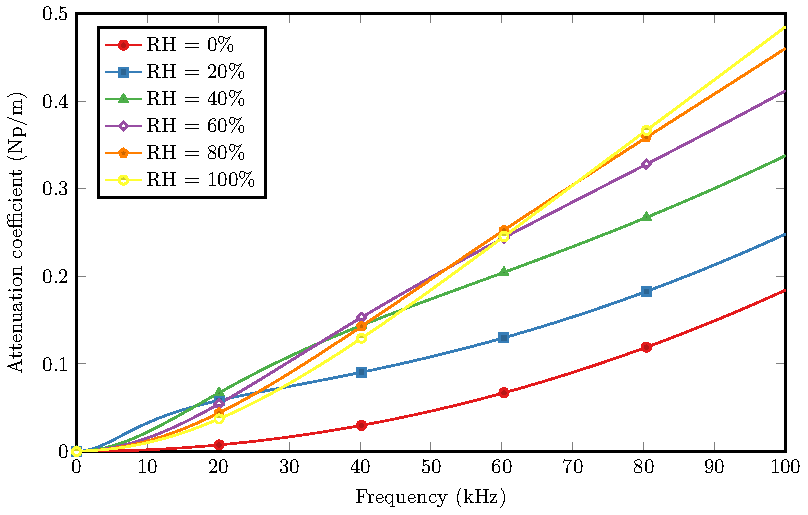
\includegraphics[width = 0.8\textwidth]{fig/AbsorpCoeff_Compare_211014A_v2.pdf}
    \caption{Attenuation coefficient at 1 atm and \revA{293.15 K ($20\celsius$)}  are shown as a function of frequency at different relative humidity (RH).}
    \label{fig:412031200}
\end{figure}


\section{Absorption distance of PALs}
The absorption distance of PALs is usually defined as the reciprocal of the sound attenuation coefficient of two ultrasonic waves \cite{Shi2013InvestigationSteerableParametric, Farias2015RayleighDistanceAbsorption}
\begin{equation}
    L\subt{a} = \frac{1}{\alpha_1+\alpha_2}\approx \frac{1}{2\alpha\subt{u}}
    \label{eq:2390jfklsdfjsd}
\end{equation}
where the approximation is valid when $\alpha_1\approx \alpha_2$.
The absorption distance at 1 atm and 293.15 K (20\celsius {}) are shown in Fig.~\ref{fig:4120312002}.

\begin{figure}[!htb]
    \centering
    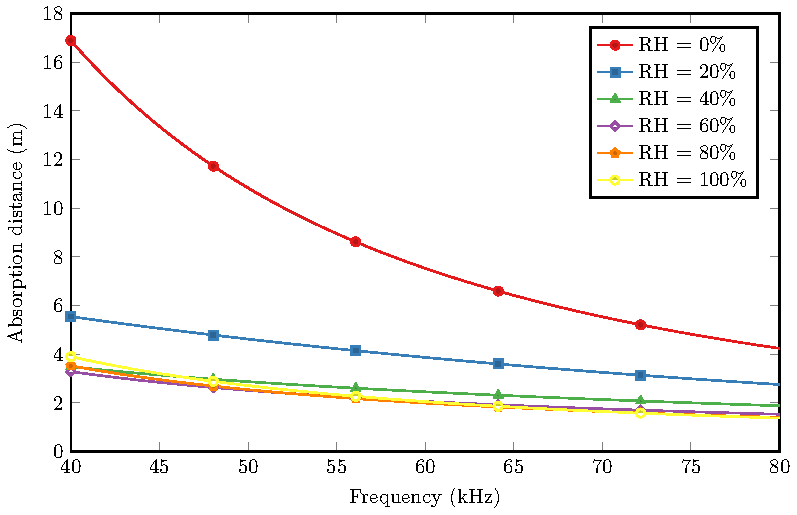
\includegraphics[width = 0.8\textwidth]{fig/AbsorpLen_demo211218A.pdf}
    \caption{Absorption distance of PALs at 1 atm and 293.15 K (20\celsius {})  are shown as a function of frequency at different relative humidity.}
    \label{fig:4120312002}
\end{figure}

